\documentclass[11pt,a4paper]{article}

\usepackage[utf8]{inputenc}
\usepackage[T1]{fontenc}
\usepackage{amsmath,amssymb,amsthm}
\usepackage{mathtools}
\usepackage{booktabs}
\usepackage{hyperref}
\usepackage{geometry}
\usepackage{enumitem}
\usepackage{listings}
\usepackage{longtable}
\usepackage{textcomp}
\usepackage{array}
\usepackage{tikz}
\usetikzlibrary{arrows.meta,positioning,calc,shapes.geometric,automata}

\geometry{margin=1in}
\setcounter{tocdepth}{2}

\newtheorem{definition}{Definition}[section]
\newtheorem{principle}[definition]{Principle}
\newtheorem{theorem}[definition]{Theorem}
\newtheorem{proposition}[definition]{Proposition}
\newtheorem{invariant}[definition]{Invariant}
\newtheorem{remark}[definition]{Remark}

\lstset{
  basicstyle=\ttfamily\small,
  columns=fullflexible,
  keepspaces=true,
  xleftmargin=2em,
  aboveskip=0.5em,
  belowskip=0.5em
}

\title{The Ledger Valuation Stack\\[6pt]
\large Pricing, Greeks, Calibration, PnL Attribution, and Temporal Orchestration\\[4pt]
\normalsize Companion Document to the Ledger Framework Specification}
\author{R.\ Delloye}
\date{March 2026 --- v1.0}

\begin{document}
\maketitle

\begin{abstract}
The Ledger framework~\cite{ledger} defines portfolio value as $V_t = \sum_u \mathrm{own}(u) \cdot P_t(u)$ and proves that PnL is path-independent.  The framework deliberately treats $P_t$ as an external input without specifying how that function is computed, validated, or delivered.

This companion document fills the gap.  Version~1.0 makes five contributions beyond the v0.2 draft.

First, it introduces a \emph{finite state machine} (FSM) for the valuation lifecycle of every unit.  Eight states---\textsc{Unpriced}, \textsc{Pricing}, \textsc{Priced}, \textsc{Explaining}, \textsc{Explained}, \textsc{Quarantined}, \textsc{Stale}, and \textsc{Failed}---govern the progression from market data arrival through pricing, PnL explain verification, and publication.  Every transition has a triggering event and a guard condition; terminal and absorbing behaviours are explicit.

Second, it formalises the \emph{Kalman filter for market data calibration}, drawing from the Calibration Manifesto~\cite{calibration_manifesto}.  The state vector (latent curve or surface parameters), observation model (market observables as functions of state), transition dynamics (driftless random walk consistent with the martingale axiom), noise structure (bid-ask-derived observation noise and process noise governing adaptation speed), and the predict-update cycle are specified.  Innovation-based gating rejects bad data; filtered estimates feed the pricing DAG as calibrated market data nodes.

Third, it reframes \emph{Greeks through the parameter-martingale lens}: a model has parameters assumed to be martingales; Greeks are partial derivatives with respect to observables, holding parameters constant.  The key insight is that ``vega'' only exists as a scalar when volatility is a single parameter (Black--Scholes); in multi-parameter models (Heston, SABR, local vol), vega is replaced by the \emph{sensitivity Jacobian}---a vector whose dimension equals the number of model parameters.  This framework is developed concretely: Black--Scholes delta versus local vol delta under a skewed surface, total gamma incorporating vanna, volga, and vega-curvature adjustments~\cite{pnl_total_gamma,total_gamma}, the toxic product boundary, the consensus protocol for multi-model disagreement, and practical computation methods (analytical, bump-and-revalue, AAD, pathwise/likelihood ratio).

Fourth, it tightens \emph{integration with the Ledger}: the price function $P(u, \mathrm{state}_t(u), \mathrm{market\_data}_t)$ is a formal definition, the lifecycle-valuation ordering protocol is embedded in the FSM, and the Taylor approximation is explicitly positioned as the price in state \textsc{Explained} between repricing cycles.

Fifth, it hardens the \emph{production architecture} with a scalability analysis: one workflow per unit at 100{,}000 units with 30-second average cadence yields 200{,}000 workflow executions per minute, within Temporal cluster capacity with horizontal scaling.

The document retains all material from v0.2 (the ValuationRecord, Pricing DAG, Temporal workflow architecture, PnL explain gate, continuous approximate pricing, valuation store, edge cases, worked examples, and lifecycle consistency) and integrates the new contributions into the existing structure.
\end{abstract}

\tableofcontents
\clearpage

%==============================================================================
\section{Introduction}
\label{sec:intro}
%==============================================================================

The Ledger framework~\cite{ledger} establishes six properties by construction: atomicity, conservation, determinism, state-sufficiency, lifecycle value invariance, and time travel.  Portfolio valuation appears in~\cite[\S4]{ledger} as:
\[
V_t = \sum_{u \in \mathcal{U}} w_t(u) \cdot P_t(u)
\]
where $w_t(u)$ is the wallet balance (or, in the generalised position model, $\mathrm{own}(u)$) and $P_t(u)$ is the price of unit $u$ at time $t$ in the reference currency.  The path-independence theorem~\cite[\S4.3]{ledger} proves that $\mathrm{PnL} = V_{t_1} - V_{t_0}$ regardless of intermediate trading activity.

The framework is deliberately agnostic to the pricing methodology: ``$P_t$ is an \emph{external input} to the framework, not computed by it''~\cite[\S4.1]{ledger}.  This is the correct architectural boundary---the ledger is a settlement and position system, not a pricing engine.  But the boundary creates five unanswered questions:

\begin{enumerate}
\item \textbf{What does $P_t(u)$ return?}  A price is not a scalar in practice.  How does structured output interact with the scalar $P_t$ of the PnL theorem?

\item \textbf{How are prices computed in dependency order?}  Dependencies form a directed acyclic graph.  How is it defined, enforced, and executed?

\item \textbf{How are new prices validated?}  PnL explain provides the mathematical foundation but not the operational pipeline.

\item \textbf{What price is available between full reprices?}  Complex instruments take seconds to minutes.  Between cycles, the risk pipeline needs a current price.

\item \textbf{What is the lifecycle of a valuation?}  From the arrival of fresh market data through pricing, verification, and publication---what states does a unit's valuation pass through, and what governs the transitions?
\end{enumerate}

This document answers all five.

\subsection{Relationship to the Ledger Specification}

This document is a companion to, not a revision of, the Ledger framework~\cite{ledger}.  It introduces no new primitives (no new move types, no new wallet structures, no changes to the conservation law).  It specifies the \emph{valuation layer} that produces the $P_t$ function consumed by the ledger's PnL computation.

\subsection{Relationship to the Reference Papers}

The PnL explain paper~\cite{pnl_explain} establishes the polynomial decomposition of price changes.  The PnL attribution and total gamma paper~\cite{pnl_total_gamma} unifies the polynomial framework with smile-adjusted sensitivities and defines the toxic product boundary.  The Calibration Manifesto~\cite{calibration_manifesto} provides the Bayesian framework for market data calibration.  The implied volatility~\cite{implied_vol} and local volatility~\cite{implied_local_vol,loc_vol} papers define the models that produce model-dependent Greeks.  The control variate paper~\cite{control_variate} specifies regression-based Monte Carlo with surrogate models.  The total gamma paper~\cite{total_gamma} derives the adjusted gamma under spot-dependent volatility.

This document operationalises all of these results within a unified valuation architecture.

\subsection{Document Roadmap}

Section~\ref{sec:fsm} defines the valuation lifecycle FSM.  Section~\ref{sec:valuation-record} defines the ValuationRecord.  Section~\ref{sec:greeks} reframes Greeks through the parameter-martingale lens, introduces the sensitivity Jacobian, develops total gamma, and specifies the consensus protocol.  Section~\ref{sec:calibration} formalises the Kalman filter for market data calibration.  Section~\ref{sec:pricing-dag} introduces the Pricing DAG.  Section~\ref{sec:temporal} specifies the Temporal workflow architecture.  Section~\ref{sec:pnl-explain} formalises PnL explain.  Section~\ref{sec:approx-pricing} introduces continuous approximate pricing.  Section~\ref{sec:valuation-store} describes the valuation store.  Section~\ref{sec:edge-cases} catalogues edge cases.  Section~\ref{sec:worked-example} traces a complete valuation cycle.  Section~\ref{sec:lifecycle-consistency} formalises lifecycle-valuation consistency.  Section~\ref{sec:scalability} provides the production scalability analysis.  Section~\ref{sec:conclusion} identifies open problems.

\clearpage
%==============================================================================
\section{The Valuation Lifecycle FSM}
\label{sec:fsm}
%==============================================================================

Every unit in the Pricing DAG has a valuation state that governs what operations are permitted and what downstream consumers can expect.  The valuation lifecycle is a finite state machine (FSM) with eight states and twelve transitions.

\subsection{States}

\begin{definition}[Valuation States]
\label{def:val-states}
The valuation lifecycle of a unit $u$ is described by a state $\sigma(u) \in \mathcal{S}$, where:
\[
\mathcal{S} = \{\textsc{Unpriced},\; \textsc{Pricing},\; \textsc{Priced},\; \textsc{Explaining},\; \textsc{Explained},\; \textsc{Quarantined},\; \textsc{Stale},\; \textsc{Failed}\}
\]
Each state has the following semantics:

\begin{center}
\small
\begin{tabular}{l p{9cm}}
\toprule
\textbf{State} & \textbf{Semantics} \\
\midrule
\textsc{Unpriced} & Unit registered in the Unit Store but never priced.  No ValuationRecord exists.  No approximate price is available.  The unit is invisible to the PnL pipeline.  This is the initial state for every newly registered unit. \\
\textsc{Pricing} & A pricing computation is in progress.  The pricer activity has been dispatched but has not yet returned.  The previous FIRM price (if any) remains current.  Approximate pricing from the previous cycle's Greeks is available. \\
\textsc{Priced} & The pricer has returned a candidate ValuationRecord.  The record has not yet been verified by PnL explain.  This is a transient state---the system immediately initiates the explain check. \\
\textsc{Explaining} & PnL explain is executing.  The candidate record is being compared against the previous FIRM record using the Taylor decomposition. \\
\textsc{Explained} & PnL explain passed.  The ValuationRecord is published to the valuation store with \texttt{quality = FIRM}.  Greeks are cached for approximate pricing.  This is the normal resting state between pricing cycles. \\
\textsc{Quarantined} & PnL explain failed: the unexplained residual exceeds tolerance.  The candidate record is held in quarantine.  The previous FIRM price remains current.  Automated retry is initiated. \\
\textsc{Stale} & The staleness timer has expired without a new pricing cycle completing.  The last FIRM price is retained with \texttt{quality = STALE}.  Downstream consumers apply prudential haircuts. \\
\textsc{Failed} & The pricer returned an error, timed out, or produced a numerically invalid result (NaN, Inf, negative price for a non-negative instrument).  Retry is initiated with backoff. \\
\bottomrule
\end{tabular}
\end{center}
\end{definition}

\noindent \textbf{Terminal states.}  There are no terminal states in the FSM during the unit's active lifecycle.  Every non-\textsc{Explained} state has at least one outgoing transition.  When the unit's lifecycle terminates (option expiry, bond maturity), the unit exits the Pricing DAG entirely; the FSM ceases to apply, and the terminal valuation is deterministic~\cite[\S7]{ledger}.

\subsection{Transitions}

\begin{definition}[Valuation Transitions]
\label{def:val-transitions}
The transition function $\delta : \mathcal{S} \times \mathcal{E} \to \mathcal{S}$ maps (current state, triggering event) to a new state, subject to guard conditions.  The transitions are:
\end{definition}

\begin{center}
\small
\begin{longtable}{r l l l l}
\toprule
\textbf{\#} & \textbf{From} & \textbf{To} & \textbf{Trigger} & \textbf{Guard} \\
\midrule
\endfirsthead
\toprule
\textbf{\#} & \textbf{From} & \textbf{To} & \textbf{Trigger} & \textbf{Guard} \\
\midrule
\endhead
T1 & \textsc{Unpriced} & \textsc{Pricing} & Market data arrives & \parbox[t]{4.5cm}{Market data fresh \textbf{and} all upstream DAG nodes have a FIRM price (or first cycle)} \\[8pt]
T2 & \textsc{Pricing} & \textsc{Priced} & Pricer returns & Pricer returns valid result \\[4pt]
T3 & \textsc{Pricing} & \textsc{Failed} & Pricer error & Pricer error, timeout, or invalid result \\[4pt]
T4 & \textsc{Priced} & \textsc{Explaining} & PnL explain invoked & Always (automatic) \\[4pt]
T5 & \textsc{Explaining} & \textsc{Explained} & Explain passes & $|\text{unexplained}| < \text{tolerance}(u)$ \\[4pt]
T6 & \textsc{Explaining} & \textsc{Quarantined} & Explain fails & $|\text{unexplained}| \geq \text{tolerance}(u)$ \\[4pt]
T7 & \textsc{Quarantined} & \textsc{Pricing} & Retry initiated & \parbox[t]{4.5cm}{Retry count $<$ max retries \textbf{and} (refreshed data available \textbf{or} alternative model available)} \\[8pt]
T8 & \textsc{Explained} & \textsc{Stale} & Staleness timer & \parbox[t]{4.5cm}{No new cycle completed within staleness threshold} \\[8pt]
T9 & \textsc{Stale} & \textsc{Pricing} & New market data & \parbox[t]{4.5cm}{Fresh market data arrives \textsc{and} upstream nodes fresh} \\[8pt]
T10 & \textsc{Failed} & \textsc{Pricing} & Retry after backoff & \parbox[t]{4.5cm}{Backoff period elapsed \textsc{and} retry count $<$ max attempts} \\[8pt]
T11 & \textsc{Quarantined} & \textsc{Stale} & Retries exhausted & \parbox[t]{4.5cm}{Retry count $=$ max retries \textbf{and} no manual override} \\[4pt]
T12 & \textsc{Failed} & \textsc{Stale} & Retries exhausted & \parbox[t]{4.5cm}{Retry count $=$ max attempts \textbf{and} no fallback model} \\[4pt]
\bottomrule
\end{longtable}
\end{center}

\noindent \textbf{Note on T1 guard.}  For the very first pricing cycle of a unit (state = \textsc{Unpriced}), the guard on upstream nodes being \textsc{Explained} is relaxed: it suffices that upstream nodes have \emph{any} FIRM price available, even from a previous cycle.  This avoids a bootstrap deadlock where no unit can be priced because none is yet \textsc{Explained}.

\subsection{FSM Diagram}

\begin{figure}[ht]
\centering
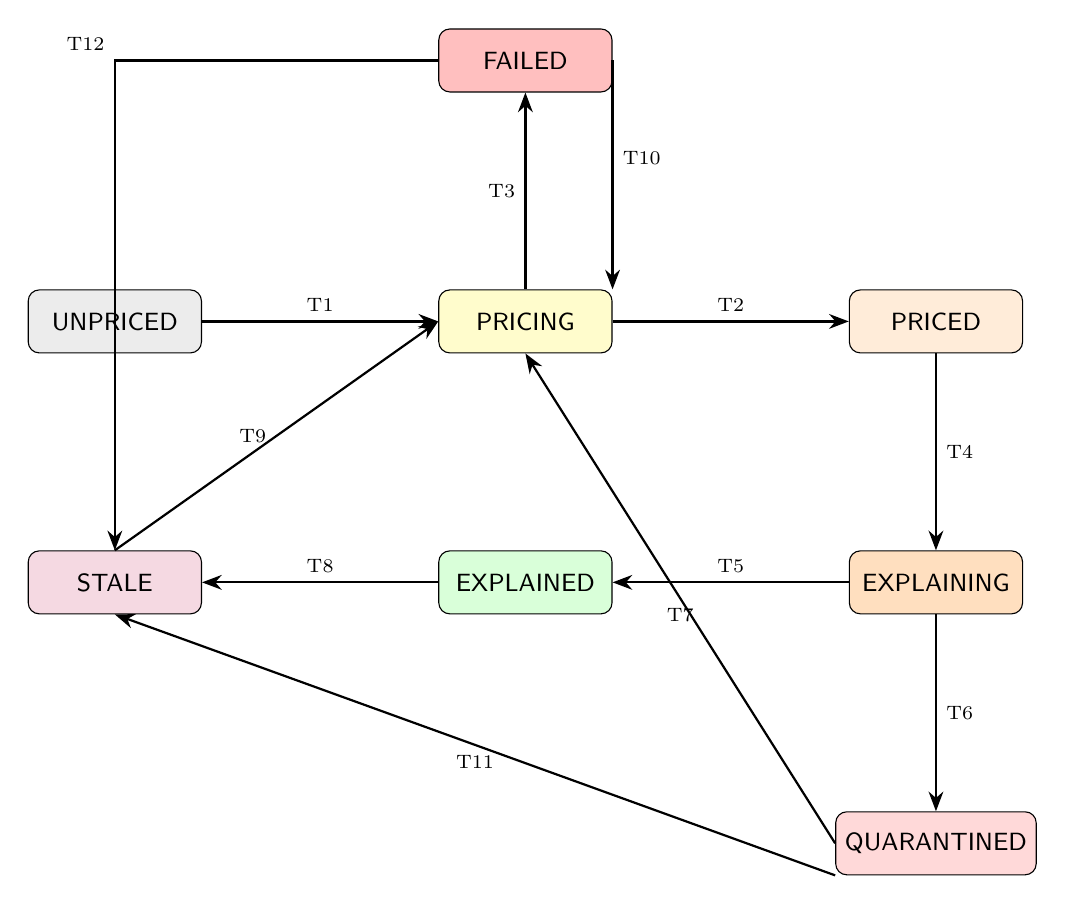
\begin{tikzpicture}[
    state/.style={draw, rounded corners, minimum width=2.2cm, minimum height=0.8cm, font=\small\sffamily, align=center},
    trans/.style={-{Stealth[length=2.5mm]}, thick, font=\scriptsize},
    every node/.append style={font=\scriptsize},
    node distance=2.5cm and 3cm,
  ]
  % States
  \node[state, fill=gray!15] (unpriced) {UNPRICED};
  \node[state, fill=yellow!20, right=of unpriced] (pricing) {PRICING};
  \node[state, fill=orange!15, right=of pricing] (priced) {PRICED};
  \node[state, fill=orange!25, below=of priced] (explaining) {EXPLAINING};
  \node[state, fill=green!15, below=of pricing] (explained) {EXPLAINED};
  \node[state, fill=red!15, below=of explaining] (quarantined) {QUARANTINED};
  \node[state, fill=red!25, above=of pricing] (failed) {FAILED};
  \node[state, fill=purple!15, left=of explained] (stale) {STALE};

  % Transitions
  \draw[trans] (unpriced) -- node[above] {T1} (pricing);
  \draw[trans] (pricing) -- node[above] {T2} (priced);
  \draw[trans] (pricing) -- node[left] {T3} (failed);
  \draw[trans] (priced) -- node[right] {T4} (explaining);
  \draw[trans] (explaining) -- node[above] {T5} (explained);
  \draw[trans] (explaining) -- node[right] {T6} (quarantined);
  \draw[trans] (quarantined.west) -- node[below] {T7} (pricing.south);
  \draw[trans] (explained) -- node[above] {T8} (stale);
  \draw[trans] (stale.north) -- node[left] {T9} (pricing.west);
  \draw[trans] (failed.east) -- node[above right] {T10} (pricing.north east);
  \draw[trans] (quarantined.south west) -- node[below] {T11} (stale.south);
  \draw[trans] (failed.west) -| node[above left] {T12} (stale.north);
\end{tikzpicture}
\caption{Valuation lifecycle FSM.  Green: normal resting state.  Yellow/orange: transient processing states.  Red: failure states.  Purple: degraded state.  Gray: initial state.}
\label{fig:fsm}
\end{figure}

\subsection{FSM and the Pricing Workflow}

The FSM is implemented within the \texttt{PricingWorkflow} (Section~\ref{sec:temporal}).  The workflow maintains the current state $\sigma(u)$ as a workflow-local variable.  Each transition is atomic: the workflow advances the state, performs the associated action, and persists the state via Temporal's durable execution.  On workflow replay, the state is recovered from the event history.

The FSM integrates with the lifecycle engine (Section~\ref{sec:lifecycle-consistency}) as follows: lifecycle events that are \emph{material} (Definition~\ref{def:repricing-class}) force the unit into \textsc{Pricing} regardless of current state, because the cached Greeks are invalid after the state change.  Non-material lifecycle events do not affect the FSM.

\subsection{FSM and the Taylor Approximation}

The Taylor approximation (Section~\ref{sec:approx-pricing}) is available \emph{only} in state \textsc{Explained}.  In this state, the last FIRM ValuationRecord provides the base price and Greeks, and current market data moves provide the perturbation.  The approximate price is:
\[
P_{\mathrm{approx}}(u, t) = P_{\mathrm{FIRM}}(u) + \langle \Delta \,|\, \Delta x(t) \rangle + \tfrac{1}{2}\langle \Delta x(t) \,|\, \Gamma \,|\, \Delta x(t) \rangle
\]
where $\Delta x(t)$ is the market data move since the last FIRM snapshot.  When the unit transitions out of \textsc{Explained} (via T8 to \textsc{Stale}, or via a lifecycle event to \textsc{Pricing}), the Taylor approximation is invalidated.

The FSM thus makes explicit what v0.2 described procedurally: the Taylor approximation is the price in state \textsc{Explained} between repricing cycles.

\clearpage
%==============================================================================
\section{The Valuation Record}
\label{sec:valuation-record}
%==============================================================================

The Ledger specification defines $P_t : \mathcal{U} \to \mathbb{R}$ as a scalar function.  In practice, the output of a pricing computation is richer.

\begin{definition}[Valuation Record]
\label{def:valuation-record}
A \emph{ValuationRecord} for unit $u$ at time $t$ is a tuple:
\begin{lstlisting}
ValuationRecord:
    unit_id:          UnitId
    timestamp:        Timestamp
    dirty_price:      Decimal       -- full market value including accrual
    clean_price:      Decimal       -- quoted price net of accrual
    accrued:          Decimal       -- dirty_price - clean_price
    greeks:           Greeks        -- model-specific sensitivity vector
    model_id:         String        -- which pricer produced this (load-bearing)
    market_data_snap: SnapshotId    -- which market data was used
    compute_ms:       Int           -- how long pricing took
    quality:          Quality       -- FIRM | INDICATIVE | APPROXIMATE
                                    --   | STALE | FAILED
    fsm_state:        ValuationState -- current FSM state at publication
\end{lstlisting}
\end{definition}

\begin{principle}[Scalar Compatibility]
\label{princ:scalar-compat}
The \texttt{dirty\_price} field IS the $P_t(u)$ of~\cite[\S4.1]{ledger}.  The path-independence theorem is preserved:
\[
\mathrm{PnL} = V_{t_1} - V_{t_0} = \sum_{u} \mathrm{own}(u) \cdot \bigl[\texttt{dirty\_price}_{t_1}(u) - \texttt{dirty\_price}_{t_0}(u)\bigr]
\]
The remaining fields are metadata that enriches the record without altering the theorem.
\end{principle}

\subsection{Quality Semantics}

The \texttt{quality} flag has five values with precise operational semantics:

\begin{center}
\small
\begin{tabular}{l p{9cm}}
\toprule
\textbf{Quality} & \textbf{Semantics} \\
\midrule
\texttt{FIRM} & Full reprice from live market data; PnL explain passed.  FSM state: \textsc{Explained}. \\
\texttt{INDICATIVE} & Full reprice completed but PnL explain tolerance exceeded, or market data from secondary source. \\
\texttt{APPROXIMATE} & Taylor expansion from the last FIRM valuation.  FSM state: \textsc{Explained} (between cycles). \\
\texttt{STALE} & Last FIRM valuation older than staleness threshold.  FSM state: \textsc{Stale}. \\
\texttt{FAILED} & Pricer failed.  FSM state: \textsc{Failed}. \\
\bottomrule
\end{tabular}
\end{center}

\subsection{Dirty Price, Clean Price, and Accrued Interest}

For instruments with accrual mechanics (bonds, loans, swaps):
\[
\texttt{dirty\_price} = \texttt{clean\_price} + \texttt{accrued}
\]
The accrued interest is computed from the unit state~\cite[\S7]{ledger}.  For instruments without accrual, \texttt{clean\_price} $=$ \texttt{dirty\_price} and \texttt{accrued} $= 0$.

\clearpage
%==============================================================================
\section{Greeks, Parameters, and the Sensitivity Jacobian}
\label{sec:greeks}
%==============================================================================

\subsection{Models, Parameters, and the Martingale Assumption}
\label{sec:model-params}

A pricing model $\mathcal{M}$ is defined by three objects:

\begin{definition}[Pricing Model]
\label{def:pricing-model}
A pricing model $\mathcal{M}$ consists of:
\begin{enumerate}[nosep]
\item A set of \emph{observables} $O = \{S, r, \ldots\}$---quantities directly measured in the market (spot price, deposit rate, exchange rate).  These move, and we see them move.
\item A set of \emph{parameters} $\Theta = \{\theta_1, \ldots, \theta_n\}$---quantities calibrated from market data (implied vol, mean reversion speed, vol-of-vol, correlation, curvature coefficients).  These are inferred, not directly observed.
\item A price function $P_\mathcal{M}(O, \Theta, T)$ that maps observables, parameters, and time to a price.
\end{enumerate}
\end{definition}

The distinction between observables and parameters is the distinction between what the model \emph{takes as given} and what the model \emph{infers}.  Spot is an observable: it trades on an exchange and has a last price.  Implied volatility is a parameter: it is backed out from option prices via an inversion of the Black--Scholes formula.  The Kalman filter in Section~\ref{sec:calibration} is the mechanism that performs this inference---it transforms raw observations $y_t$ into calibrated parameter estimates $x_{t|t}$.

\begin{principle}[The Martingale Assumption on Parameters]
\label{princ:martingale-params}
The model assumes that its parameters are martingales:
\begin{equation}\label{eq:param-martingale}
\mathbb{E}[\Theta(t + \mathrm{d}t) \mid \mathcal{F}_t] = \Theta(t)
\end{equation}
That is: the best forecast of tomorrow's parameter value is today's parameter value.  This is \emph{not} the claim that parameters are constant.  Parameters can and do change.  But the model prices \emph{as if} the current parameter values are the best estimate of future parameter values.
\end{principle}

\noindent This is the same assumption that underpins the driftless transition model in the Kalman filter (Eq.~\ref{eq:transition}): $x_t = x_{t-1} + w_t$ with $\mathbb{E}[x_t \mid \mathcal{I}_{t-1}] = x_{t-1}$.  It is also Axiom~A5 of the Calibration Manifesto~\cite{calibration_manifesto}: the posterior mean is a martingale.  The assumption appears in three places---the transition model, the pricing model, and the Greek computation---because it \emph{is} the same assumption.

\subsection{Greeks as Parameter-Invariant Sensitivities}
\label{sec:greeks-invariant}

A Greek is a partial derivative of the price function with respect to an observable, holding all parameters at their current values.

\begin{definition}[Greek]
\label{def:greek}
Let $\mathcal{M}$ be a pricing model with price function $P_\mathcal{M}(O, \Theta, T)$.  A \emph{Greek} with respect to observable $O_i$ is:
\[
\left.\frac{\partial P_\mathcal{M}}{\partial O_i}\right|_{\Theta}
\]
The subscript $|_{\Theta}$ is essential: it asserts that all model parameters are held at their current values.  This is well-defined \emph{because} parameters are martingales---bumping an observable does not, in the model's worldview, change the parameters.
\end{definition}

\noindent Delta, gamma, rho, and theta are Greeks in this sense: they are partial derivatives with respect to observables ($S$, $r$, $t$), holding all model parameters constant.  These are well-defined for every model.

But ``vega''---the sensitivity to volatility---requires a more careful treatment.

\subsection{The Vanishing Vega Problem}
\label{sec:vanishing-vega}

In Black--Scholes, volatility $\sigma$ is a single parameter.  The quantity $\partial P / \partial \sigma$ is well-defined: there is one number to bump, and the derivative is a scalar.  This is what traders call ``vega.''

But in any model where volatility is governed by multiple parameters, the scalar ``vega'' does not exist.  It is replaced by a \emph{vector} of parameter sensitivities whose dimension depends on the model:

\begin{center}
\small
\renewcommand{\arraystretch}{1.4}
\begin{tabular}{@{}l l l p{5cm}@{}}
\toprule
\textbf{Model} & \textbf{Vol parameters} & \textbf{Dim} & \textbf{Vol sensitivities} \\
\midrule
Black--Scholes & $\sigma_{\mathrm{imp}}$ & 1 & $\frac{\partial P}{\partial \sigma_{\mathrm{imp}}}$ (scalar ``vega'') \\[4pt]
Heston & $v_0, \kappa, \theta, \xi, \rho$ & 5 & $\frac{\partial P}{\partial v_0},\; \frac{\partial P}{\partial \kappa},\; \frac{\partial P}{\partial \theta},\; \frac{\partial P}{\partial \xi},\; \frac{\partial P}{\partial \rho}$ \\[4pt]
SABR & $\alpha, \beta, \rho, \nu$ & 4 & $\frac{\partial P}{\partial \alpha},\; \frac{\partial P}{\partial \beta},\; \frac{\partial P}{\partial \rho},\; \frac{\partial P}{\partial \nu}$ \\[4pt]
Local vol & $\sigma_{\mathrm{loc}}(K_i, T_j)$ grid & $N_K \times N_T$ & $\frac{\partial P}{\partial \sigma_{\mathrm{loc}}(K_i, T_j)}$ (a matrix) \\[4pt]
Kernel vol~\cite{implied_vol} & $\sigma_0, s_0, c_1, \ldots, c_n$ & $n+2$ & $\frac{\partial P}{\partial \sigma_0},\; \frac{\partial P}{\partial s_0},\; \frac{\partial P}{\partial c_1},\; \ldots$ \\[2pt]
\bottomrule
\end{tabular}
\end{center}

\begin{principle}[Vega is Model-Specific]
\label{princ:vega-model-specific}
``Vega'' is not a universal Greek.  It is a model-specific sensitivity whose dimension equals the number of volatility-related parameters in the model.  In Black--Scholes, vega is a scalar.  In Heston, it is a 5-vector.  In local vol, it is a matrix.  The scalar ``vega'' that Bloomberg reports is the Black--Scholes vega---$\partial P / \partial \sigma_{\mathrm{imp}}$---regardless of which model priced the option.  This is a \emph{convention}, not a fundamental quantity.
\end{principle}

\noindent The practical consequences are immediate.  If a risk system reports a single ``vega'' number for a position priced with Heston, it has projected a 5-dimensional sensitivity onto a single axis.  The projection discards information about how the position responds to changes in mean reversion, vol-of-vol, or correlation.  The discarded information becomes unexplained PnL.

\subsection{The Sensitivity Jacobian}
\label{sec:jacobian}

The general framework replaces the scalar ``vega'' with the full parameter Jacobian.

\begin{definition}[Sensitivity Jacobian]
\label{def:jacobian}
For a model $\mathcal{M}$ with parameters $\Theta = (\theta_1, \ldots, \theta_n)$, the \emph{sensitivity Jacobian} is the row vector:
\begin{equation}\label{eq:jacobian}
J = \left(\frac{\partial P}{\partial \theta_1},\; \frac{\partial P}{\partial \theta_2},\; \ldots,\; \frac{\partial P}{\partial \theta_n}\right) \in \mathbb{R}^{1 \times n}
\end{equation}
This is the gradient of price with respect to all model parameters, holding observables constant.
\end{definition}

\noindent The PnL decomposition becomes:
\begin{equation}\label{eq:pnl-jacobian}
\boxed{
\Delta P \;\approx\; \underbrace{\delta \cdot \Delta S}_{\text{delta PnL}} \;+\; \underbrace{J \cdot \Delta\Theta}_{\text{parameter PnL}} \;+\; \underbrace{\tfrac{1}{2}\,\Gamma \cdot (\Delta S)^2}_{\text{gamma PnL}} \;+\; \underbrace{\Theta_{\text{decay}} \cdot \Delta t}_{\text{theta PnL}} \;+\; \varepsilon
}
\end{equation}
where $\Delta\Theta = \Theta_{t} - \Theta_{t-1}$ is the observed change in calibrated parameters between two valuation times, and $J \cdot \Delta\Theta = \sum_{i=1}^{n} \frac{\partial P}{\partial \theta_i}\,\Delta\theta_i$ is the \emph{parameter PnL}.

The ``unexplained'' residual $\varepsilon$ now captures only higher-order terms, cross-gamma terms, and model error.  The parameter PnL---which was previously \emph{inside} the unexplained term when using scalar vega---is now explicitly attributed to each parameter that moved.

\begin{remark}[The scalar vega as a projection]
\label{rem:vega-projection}
The scalar ``vega'' reported by Bloomberg is the inner product $J \cdot \hat{e}_{\sigma}$, where $\hat{e}_{\sigma}$ is the unit vector in the direction of a parallel shift of the entire implied vol surface.  It is a projection of the full Jacobian $J \in \mathbb{R}^n$ onto a specific direction in parameter space.  This projection is useful as a summary statistic but discards all information about non-parallel moves (skew steepening, curvature changes, term structure rolling).
\end{remark}

\subsection{Why the Invariant Matters for PnL}
\label{sec:invariant-pnl}

Different models have different parameter sets $\Theta$, therefore different Jacobians $J$, and therefore different PnL decompositions.

\paragraph{Black--Scholes.}  $\Theta = \{\sigma_{\mathrm{imp}}\}$, so $J = (\nu)$ is the scalar vega.  The model holds $\sigma_{\mathrm{imp}}$ constant.  But implied volatility is not constant---it has skew and term structure, and the skew moves with spot.  The unexplained term includes the skew moving with spot (the ``skew delta''), the convexity changes in the smile, and any term structure rolling.

\paragraph{Local volatility.}  $\Theta = \{\sigma_{\mathrm{loc}}(K_i, T_j)\}$ is the entire local vol grid.  When delta is computed by bumping spot, the local vol at the new spot is different (because the local vol surface, derived from the implied vol surface via Dupire's formula~\cite{loc_vol,implied_local_vol}, encodes the smile).  Local vol delta already accounts for how the vol surface shifts with spot under sticky-local-vol dynamics---the model's invariant is closer to empirical behaviour than Black--Scholes, so the unexplained PnL is typically smaller.

\paragraph{Heston.}  $\Theta = \{v_0, \kappa, \theta, \xi, \rho\}$.  The Jacobian has five components.  The parameter closest to ``vega'' is $\partial P / \partial v_0$ (sensitivity to initial variance).  But $\partial P / \partial \theta$ (long-run variance), $\partial P / \partial \xi$ (vol-of-vol), and $\partial P / \partial \rho$ (spot-vol correlation) also affect the option price through distinct channels.  Reporting only $\partial P / \partial v_0$ as ``vega'' discards the sensitivity to correlation and vol-of-vol changes.

\paragraph{The fundamental insight.}  The model with the richest parameter set that still matches market behaviour produces the most informative Jacobian and the smallest unexplained PnL.  Under-parameterised models (Black--Scholes) lump multiple distinct risks into the unexplained residual.  Over-parameterised models (too many local vol nodes) create numerical instability without reducing the residual.  The Jacobian dimension is a design choice with direct PnL consequences.

\subsection{Black--Scholes Delta vs.\ Local Vol Delta: A Concrete Comparison}
\label{sec:bs-vs-lv}

Consider an at-the-money NVDA call with $S = K = 900$, $T = 0.25$, $r = 5\%$, and a market implied volatility of 42\%.  The equity skew is typical: deep OTM puts trade at higher implied vol than ATM.

\paragraph{Black--Scholes ($\Theta = \{\sigma_{\mathrm{imp}}\}$, held constant).}  The model assumes a flat, constant volatility surface.  The delta is $\delta_{\mathrm{BS}} = N(d_1)$ where $d_1$ incorporates the single ATM implied vol.  For our parameters:
\[
\delta_{\mathrm{BS}} = N\!\left(\frac{\ln(900/900) + (0.05 + 0.42^2/2) \times 0.25}{0.42\sqrt{0.25}}\right) = N(0.164) \approx 0.565
\]
This is the sensitivity of price to spot \emph{if you believe the vol parameters do not move when spot moves}.  Nobody believes this.

\paragraph{Local volatility ($\Theta = \{\sigma_{\mathrm{loc}}(K,T)\}$ surface, held constant).}  The local vol surface $\sigma_{\mathrm{loc}}(S, t)$ is derived from the full implied volatility smile via the Dupire formula~\cite{loc_vol,implied_local_vol}:
\[
\sigma_{\mathrm{loc}}^2(m, T) = \sigma^2 \frac{1 + 2\frac{T}{\sigma}\frac{\partial \sigma}{\partial T}}{1 - 2\frac{m}{\sigma}\frac{\partial \sigma}{\partial m} + \left(\frac{m^2}{\sigma^2} - \frac{\sigma^2 T^2}{4}\right)\left(\frac{\partial \sigma}{\partial m}\right)^2 + \sigma T \frac{\partial^2 \sigma}{\partial m^2}}
\]
When delta is computed by bumping the spot in a local vol model, the vol surface \emph{moves with the spot}: as $S$ increases, the option becomes more in-the-money, and the local vol at the new spot is lower (because of the negative equity skew).  This partial offset reduces the effective delta:
\[
\delta_{\mathrm{LV}} \approx 0.541
\]

\paragraph{The difference matters.}  The delta difference $\delta_{\mathrm{BS}} - \delta_{\mathrm{LV}} \approx 0.024$ (2.4 delta points) is material for hedging.  For a position of 1{,}000 contracts at \$100 multiplier, the hedge difference is $0.024 \times 1{,}000 \times 100 \times 900 = \$2{,}160{,}000$ in notional---a significant mishedge.

The root cause is the parameter difference: Black--Scholes has one vol parameter; local vol parameterises the entire surface.  When spot moves, local vol holds its richer parameter set constant, which implicitly adjusts implied vol according to the smile.  If the market's empirical dynamics are closer to sticky local vol (which they typically are for equities), then $\delta_{\mathrm{LV}}$ is the better hedge.  The \texttt{model\_id} field on the ValuationRecord tells risk managers which delta---and which parameter set---they are looking at.

\subsection{Total Delta: Incorporating Empirical Parameter-Spot Dependence}
\label{sec:total-delta}

The martingale assumption says that parameters do not move \emph{in expectation}.  But empirically, when spot moves, the vol surface also moves---there is a statistical dependence $\partial \theta_i / \partial S$ that is \emph{not} part of any model's dynamics but is observed in the data.

The \emph{total delta} captures both the model's partial delta and this empirical correction:
\begin{equation}\label{eq:total_delta}
\boxed{\delta_{\text{total}} = \underbrace{\left.\frac{\partial P}{\partial S}\right|_{\Theta}}_{\text{partial delta}} + \underbrace{\sum_{i=1}^{n} \frac{\partial P}{\partial \theta_i} \cdot \frac{\partial \theta_i}{\partial S}}_{\text{parameter response to spot}}}
\end{equation}

The first term is the partial delta (the model's invariant assumption: parameters do not move).  The second term is the ``skew delta''---how the price changes because parameters \emph{empirically} respond to spot moves.  The terms $\partial \theta_i / \partial S$ are \emph{not} model-derived; they come from observing how calibrated parameters change when spot changes.

In the simplest case---Black--Scholes with one vol parameter---this reduces to~\cite{pnl_total_gamma,total_gamma}:
\begin{equation}\label{eq:total_delta_bs}
\frac{dP}{dS} = \Delta + \text{Vega} \cdot \frac{d\sigma}{dS}
\end{equation}
where the ``skew delta'' term $\text{Vega} \cdot d\sigma/dS$ vanishes only if $\sigma$ is truly independent of $S$.

A model that already captures the spot-vol correlation in its dynamics (like local vol or Heston with $\rho \neq 0$) will have a partial delta closer to the total delta.  Black--Scholes, which assumes zero spot-vol correlation, will have a large skew correction.

\subsection{Total Gamma Under Smile-Dependent Volatility}
\label{sec:total-greeks}

When implied volatility depends on spot price through the smile, the classical partial-derivative gamma (computed holding $\sigma$ constant) understates the true convexity.  The total gamma incorporates the indirect effect of spot on price through volatility~\cite{pnl_total_gamma,total_gamma}:

\begin{equation}\label{eq:total_gamma}
\boxed{\Gamma_{\text{total}} = \Gamma + 2\,\text{Vanna} \cdot \frac{d\sigma}{dS} + \text{Volga} \cdot \left(\frac{d\sigma}{dS}\right)^{\!2} + \text{Vega} \cdot \frac{d^2\sigma}{dS^2}}
\end{equation}
Each term has a transparent origin:
\begin{center}
\renewcommand{\arraystretch}{1.3}
\begin{tabular}{ll}
$\Gamma$ & direct spot convexity (partial gamma, parameters held constant) \\
$2\,\text{Vanna}\cdot\sigma'$ & cross-coupling of spot and vol (two chain-rule pathways) \\
$\text{Volga}\cdot(\sigma')^2$ & vol convexity channelled through smile slope \\
$\text{Vega}\cdot\sigma''$ & price-vol sensitivity weighted by smile curvature
\end{tabular}
\end{center}

\noindent This is the total second derivative of price with respect to spot, including the effect of vol parameters moving with spot.  Using $\Gamma_{\text{total}}$ instead of $\Gamma_{\text{partial}}$ in the second-order PnL term captures the vol-spot correlation and shrinks the unexplained residual.

\subsubsection{Volatility Decomposition: ATM and Smile}

In practice~\cite{pnl_total_gamma,total_gamma}, $\sigma(S)$ is modelled as:
\begin{equation}\label{eq:vol_decomp}
\sigma(S) = \sigma_{\text{ATM}}(m) + \sigma_{\text{smile}}(k)
\end{equation}
where $m = \ln(S/S_0)$ is the log-moneyness of spot relative to a pivot and $k = \ln(K/S)$ is the log-moneyness of the strike relative to spot.  The key observation is that $m$ and $k$ respond oppositely to spot moves: $dm/dS = +1/S$, $dk/dS = -1/S$.

The total first derivative of implied vol with respect to spot is:
\begin{equation}\label{eq:dsigma_dS}
\frac{d\sigma}{dS} = \frac{\sigma'_{\text{ATM}}(m) - \sigma'_{\text{smile}}(k)}{S}
\end{equation}
and the vega-curvature contribution is:
\begin{equation}\label{eq:vega_d2sigma}
\text{Vega} \cdot \frac{d^2\sigma}{dS^2} = \frac{\text{Vega}}{S^2}\bigl[\sigma''_{\text{ATM}}(m) - \sigma'_{\text{ATM}}(m) + \sigma''_{\text{smile}}(k) + \sigma'_{\text{smile}}(k)\bigr]
\end{equation}
Every quantity in this expression is observable or computable from the volatility surface model~\cite{implied_vol,implied_local_vol}.

\subsection{PnL Attribution with the Jacobian}
\label{sec:total-greeks-pnl}

The polynomial PnL framework~\cite{pnl_explain,pnl_total_gamma} provides the \emph{form} of the decomposition; the Jacobian and total Greeks provide the \emph{content}.  The full PnL attribution is:
\begin{equation}\label{eq:pnl-full}
\boxed{
\Delta P = \underbrace{\delta \cdot \Delta S}_{\text{delta}} + \underbrace{J \cdot \Delta\Theta}_{\text{parameter}} + \underbrace{\tfrac{1}{2}\,\Gamma \cdot (\Delta S)^2}_{\text{gamma}} + \underbrace{\Theta_{\text{decay}} \cdot \Delta t}_{\text{theta}} + \underbrace{\varepsilon}_{\text{unexplained}}
}
\end{equation}

The parameter PnL $J \cdot \Delta\Theta$ is the sum over all model parameters of their sensitivity times their observed change.  For a Black--Scholes model, this is $\nu \cdot \Delta\sigma_{\mathrm{imp}}$.  For Heston, it is $\frac{\partial P}{\partial v_0}\Delta v_0 + \frac{\partial P}{\partial \kappa}\Delta\kappa + \frac{\partial P}{\partial \theta}\Delta\theta + \frac{\partial P}{\partial \xi}\Delta\xi + \frac{\partial P}{\partial \rho}\Delta\rho$.  For the kernel vol model~\cite{implied_vol}, it is $\frac{\partial P}{\partial \sigma_0}\Delta\sigma_0 + \frac{\partial P}{\partial s_0}\Delta s_0 + \sum_i \frac{\partial P}{\partial c_i}\Delta c_i$.

The unexplained residual $\varepsilon$ now captures only:
\begin{itemize}[nosep]
\item Higher-order Taylor terms (cubic and beyond)
\item Cross-gamma terms ($\partial^2 P / \partial S \partial \theta_i$, i.e., vanna, charm)
\item Model error (the model's price function does not perfectly reproduce the market)
\end{itemize}

When $\sigma = \sigma(S)$, the gradient and Hessian in the polynomial PnL identity must be the total derivatives:
\begin{equation}\label{eq:unified}
P(S_2) - P(S_1) = \frac{1}{2}\!\left(\frac{dP}{dS}\bigg|_{S_2} + \frac{dP}{dS}\bigg|_{S_1}\right) h \;-\; \frac{1}{12}\!\left(\frac{d^2P}{dS^2}\bigg|_{S_2} - \frac{d^2P}{dS^2}\bigg|_{S_1}\right) h^2
\end{equation}
Using partial Greeks in this formula---omitting the smile adjustments---produces a spurious unexplained residual equal to the PnL arising from the violated martingale assumption on parameters.

\begin{remark}[Unexplained PnL as parameter martingale violation]
\label{rem:unexplained-invariant}
Let $\delta_{\text{partial}}$ denote the partial delta (parameters held constant) and $\delta_{\text{total}}$ the total delta accounting for the empirical $\partial\Theta/\partial S$.  Over a spot move $\Delta S$, the hedge error from using $\delta_{\text{partial}}$ is:
\[
(\delta_{\text{total}} - \delta_{\text{partial}}) \cdot \Delta S = \sum_i \frac{\partial P}{\partial \theta_i} \cdot \frac{\partial \theta_i}{\partial S} \cdot \Delta S
\]
This is exactly the PnL arising from the model's martingale assumption ($\partial\theta_i/\partial S = 0$) being violated ($\theta_i$ moved with spot).  The Jacobian framing makes the source of every component of unexplained PnL transparent.
\end{remark}

\subsection{The Toxic Product Boundary}
\label{sec:toxic}

The cubic polynomial assumption is a deliberate risk management boundary~\cite{pnl_total_gamma}.

\begin{definition}[Toxic product]
\label{def:toxic}
A derivative product is \emph{toxic} if the residual $|R(x_1,x_2)| = |[P(x_2) - P(x_1)] - [P_3(x_2) - P_3(x_1)]| \geq \varepsilon$ for a tolerance $\varepsilon$ over plausible market moves, where $P_3$ is the degree-three Taylor polynomial.
\end{definition}

Within the non-toxic boundary, the third derivative $\Lambda = P'''$ is constant, $\Gamma$ is linear, and $\Delta$ is quadratic.  Every PnL identity is \emph{exact}---not approximate.  Products breaching the boundary (e.g., digital options near expiry, barrier options near trigger) exhibit sensitivity structures that cannot be hedged at standard rebalancing frequencies.  The cubic residual serves as a diagnostic: a large unexplained PnL signals that the product lies outside the boundary of manageable risk.

\subsection{The Consensus Problem: Multiple Models}
\label{sec:consensus}

When multiple models are run on the same instrument, they produce different Jacobians because their parameter sets differ.  This creates four operational questions, each with a distinct answer:

\begin{enumerate}
\item \textbf{Which delta do you hedge with?}  Use the primary model---the one whose parameter set best matches empirical dynamics.  For equities with material skew, this is typically calibrated local vol or a calibrated stochastic vol model.  The primary model is designated per instrument class and calibrated to the live vol surface.

\item \textbf{Which Greeks do you use for PnL explain?}  The \emph{same} model that produced the price (model-consistent Jacobian).  Mixing models---using model $\mathcal{M}_1$'s Jacobian to explain model $\mathcal{M}_2$'s price change---creates a spurious unexplained residual that is a model artefact, not a market phenomenon (Remark~\ref{rem:model-consistency}).

\item \textbf{Which price do you report?}  The primary model's price.  The model risk reserve equals the maximum price difference across approved models:
\[
\text{ModelReserve}(u, t) = \max_{i,j} |P_{\mathcal{M}_i}(u, t) - P_{\mathcal{M}_j}(u, t)|
\]

\item \textbf{Which Greeks do you use for risk limits?}  The most conservative---largest absolute delta for delta limits, largest VaR for capital.  This ensures that limits are not breached by model choice.
\end{enumerate}

\noindent Firms typically maintain:
\begin{itemize}[nosep]
\item A \emph{primary model} (e.g., calibrated local vol) for hedging and official PnL.
\item A \emph{secondary model} (e.g., SABR) for model risk assessment.
\item A \emph{stress model} (e.g., Black--Scholes with shocked vol) for regulatory capital.
\end{itemize}

\noindent The valuation store holds one ValuationRecord per \texttt{(unit, timestamp, model)}, so all sets of Greeks coexist.

\subsection{Practical Computation of Greeks}
\label{sec:greek-computation}

Greeks---both observable sensitivities and the parameter Jacobian---are computed by one of four methods, each with different trade-offs:

\paragraph{Analytical.}  Available for Black--Scholes and a few other closed-form models.  Fast ($<$1ms) but limited to models with closed-form price functions.  Delta, gamma, vega, theta, rho all have closed-form expressions in Black--Scholes.

\paragraph{Bump-and-revalue.}  General-purpose.  Bump each input by $\varepsilon$, reprice, compute the central difference:
\[
\frac{\partial P}{\partial \theta_i} \approx \frac{P(\theta_i + \varepsilon) - P(\theta_i - \varepsilon)}{2\varepsilon}
\]
For the full Jacobian with $n$ parameters plus $k$ observables: $2(n+k)$ reprices.  For a Heston model ($n=5$, $k=2$): 14 reprices.  For a Monte Carlo pricer at 10 seconds per call, full Jacobian computation takes 2--4 minutes.

\paragraph{Adjoint algorithmic differentiation (AAD).}  Computes the \emph{entire} Jacobian---all observable sensitivities and all parameter sensitivities---in one backward pass through the pricing algorithm.  Cost: approximately $3$--$4\times$ the base price computation, \emph{regardless of the number of parameters}.  This makes AAD particularly valuable for models with many parameters (local vol grid, kernel vol coefficients).

\paragraph{Pathwise and likelihood ratio methods (Monte Carlo).}  Alternatives to bump-and-revalue for MC pricers.  The pathwise method differentiates the payoff along each simulated path; the likelihood ratio method differentiates the probability measure rather than the payoff.  Each has bias/variance trade-offs: pathwise is unbiased for smooth payoffs but fails at discontinuities (digitals); likelihood ratio handles discontinuities but has higher variance.

\noindent Greek and Jacobian computation is a separate Temporal activity from the base price (Section~\ref{sec:temporal}), with its own timeout and retry policy.

\subsection{Greeks Structures by Instrument Class}
\label{sec:greek-structures}

The \texttt{greeks} field of the ValuationRecord is a tagged union whose structure is model-dependent.  This is a direct consequence of Principle~\ref{princ:vega-model-specific}: the dimension of the sensitivity vector equals $|\text{observables}| + |\text{parameters}|$, which varies by model.

\begin{lstlisting}
Greeks = BSOptionGreeks | HestonOptionGreeks | LocalVolGreeks
       | SABROptionGreeks | KernelVolGreeks
       | IRSGreeks | BondGreeks | FuturesGreeks | CashGreeks
\end{lstlisting}

\subsubsection{Black--Scholes Option Greeks ($\dim\Theta = 1$)}
\begin{lstlisting}
BSOptionGreeks:
    model_id:       "black_scholes"
    invariant:      "sigma_imp"
    method:         Method     -- ANALYTICAL | BUMP | AAD | PATHWISE
    bump_size:      Decimal?   -- epsilon used (for BUMP method)
    -- Observable sensitivities
    delta:          Decimal    -- dP/dS, holding sigma_imp constant
    gamma:          Decimal    -- d^2P/dS^2
    theta:          Decimal    -- dP/dt (per calendar day)
    rho:            Decimal    -- dP/dr
    -- Parameter Jacobian (dim = 1)
    vega:           Decimal    -- dP/d(sigma_imp): the scalar "vega"
    -- Cross-sensitivities (for total gamma computation)
    vanna:          Decimal    -- d^2P/(dS d(sigma_imp))
    volga:          Decimal    -- d^2P/d(sigma_imp)^2
\end{lstlisting}

\subsubsection{Heston Option Greeks ($\dim\Theta = 5$)}
\begin{lstlisting}
HestonOptionGreeks:
    model_id:       "heston"
    invariant:      "heston_params"
    method:         Method         bump_size:  Decimal?
    -- Observable sensitivities
    delta:          Decimal        gamma:      Decimal
    theta:          Decimal        rho_rate:   Decimal    -- dP/dr
    -- Parameter Jacobian (dim = 5)
    v0_sens:        Decimal    -- dP/d(v0): closest analogue to BS vega
    kappa_sens:     Decimal    -- dP/d(kappa): mean reversion sensitivity
    theta_long_sens:Decimal    -- dP/d(theta): long-run variance sens.
    xi_sens:        Decimal    -- dP/d(xi): vol-of-vol sensitivity
    rho_sens:       Decimal    -- dP/d(rho): spot-vol correlation sens.
\end{lstlisting}

\subsubsection{SABR Option Greeks ($\dim\Theta = 4$)}
\begin{lstlisting}
SABROptionGreeks:
    model_id:       "sabr"
    invariant:      "sabr_params"
    method:         Method         bump_size:  Decimal?
    -- Observable sensitivities
    delta:          Decimal        gamma:      Decimal
    theta:          Decimal        rho_rate:   Decimal
    -- Parameter Jacobian (dim = 4)
    alpha_sens:     Decimal    -- dP/d(alpha): closest to BS vega
    beta_sens:      Decimal    -- dP/d(beta): backbone sensitivity
    rho_sens:       Decimal    -- dP/d(rho): correlation sensitivity
    nu_sens:        Decimal    -- dP/d(nu): vol-of-vol sensitivity
\end{lstlisting}

\subsubsection{Local Vol / Kernel Vol Greeks ($\dim\Theta = N_K \times N_T$ or $n+2$)}
\begin{lstlisting}
LocalVolGreeks:
    model_id:       "local_vol" | "kernel_vol"
    invariant:      "sigma_loc_surface" | "kernel_params"
    method:         Method         bump_size:  Decimal?
    -- Observable sensitivities
    delta:          Decimal        gamma:      Decimal
    theta:          Decimal        rho_rate:   Decimal
    -- Parameter Jacobian (dim = grid size or kernel count + 2)
    bucket_vegas:   Map<(Strike, Expiry), Decimal>
                    -- dP/d(sigma_loc(K_i,T_j)) for each grid point
                    -- OR dP/d(c_i) for each kernel coefficient
\end{lstlisting}
The bucket vegas form a matrix (or tensor) of sensitivities.  For a typical equity surface with 10 strikes and 8 expiries, this is an 80-element Jacobian per instrument.  The ``parallel vega'' (sensitivity to shifting the entire surface by 1 vol point) is the sum of all bucket vegas.

\subsubsection{IRS Greeks}
\begin{lstlisting}
IRSGreeks:
    model_id:           String
    dv01:               Decimal
    convexity:          Decimal
    key_rate_durations: Map<Tenor, Decimal>
\end{lstlisting}
The key rate durations are the interest rate Jacobian: $\partial P / \partial r_\tau$ for each tenor $\tau$.  PnL explain: $\text{explained} \approx \sum_\tau \mathrm{KRD}_\tau \cdot \Delta r_\tau + \frac{1}{2} \cdot \mathrm{convexity} \cdot (\Delta r_{\text{par}})^2$.

\subsubsection{Bond Greeks}
\begin{lstlisting}
BondGreeks:
    model_id:           String
    modified_duration:  Decimal
    convexity:          Decimal
    dv01:               Decimal
\end{lstlisting}

\clearpage
%==============================================================================
\section{Kalman Filter for Market Data Calibration}
\label{sec:calibration}
%==============================================================================

The pricing DAG requires calibrated market data: yield curves, volatility surfaces, credit curves, and correlation parameters.  Raw market observables---swap rates, cap prices, option prices, bond yields---must be transformed into calibrated parameter vectors that satisfy no-arbitrage constraints.  The Calibration Manifesto~\cite{calibration_manifesto} provides the Bayesian framework; this section specifies the Kalman filter implementation that feeds calibrated data into the valuation engine.

\subsection{State Vector}

\begin{definition}[Calibration State]
\label{def:cal-state}
The calibration state is a latent parameter vector $x_t \in \mathbb{R}^d$ representing the current market state.  Examples:
\begin{center}
\small
\begin{tabular}{l l l}
\toprule
\textbf{Calibrated object} & \textbf{State vector $x_t$} & \textbf{Dimension $d$} \\
\midrule
USD yield curve & Zero rates at tenors 1M,3M,6M,1Y,...,30Y & 12--15 \\
Equity vol surface (per expiry) & ATM vol, skew, curvature coefficients $(\sigma_0, s_0, c_1, \ldots, c_n)$ & 5--11 \\
Credit hazard curve & Hazard rates at 1Y,3Y,5Y,7Y,10Y & 5 \\
FX vol surface & ATM vol, risk reversal, butterfly per expiry & 3--5 per expiry \\
\bottomrule
\end{tabular}
\end{center}
\end{definition}

\noindent For the implied volatility model~\cite{implied_vol,implied_local_vol}, the state vector at each expiry is the parameter ket $|\beta\rangle = (\sigma_0, s_0, c_1, \ldots, c_n)^\top$, where $\sigma_0$ is the ATM vol, $s_0$ the ATM skew, and $c_i$ the curvature coefficients of the Epanechnikov kernel decomposition.  The implied vol is $\sigma(m) = \langle\phi(m)|\beta\rangle$, linear in the parameters---enabling exact Kalman updates without linearisation.

\subsection{Transition Dynamics}

Consistent with Axiom~A5 of~\cite{calibration_manifesto} (posterior mean is a martingale), the transition model is driftless:
\begin{equation}\label{eq:transition}
x_t = x_{t-1} + w_t, \qquad w_t \sim \mathcal{N}(0, Q)
\end{equation}
where $Q$ is the process noise covariance.  The transition matrix is the identity: $A = I_d$.  This ensures:
\[
\mathbb{E}[x_t \mid I_{t-1}] = x_{t-1}
\]
Parameters move only because new information arrives.  The covariance $Q$ controls how fast the state adapts to new observations: large $Q$ allows rapid adaptation (suitable for volatile markets); small $Q$ produces smoother, more stable curves.

\paragraph{Process noise calibration.}  $Q$ is diagonal or near-diagonal for yield curves (tenor-by-tenor variance).  For vol surfaces, $Q$ may encode correlation between ATM vol and skew parameters.  Typical daily process noise standard deviations: 1--3~bp for yield curve nodes, 0.5--1.5~vol points for equity ATM vol, 0.1--0.3 for skew parameters.

\subsection{Observation Model}

At knowledge time $t$, a vector of market observables $y_t \in \mathbb{R}^{m_t}$ is observed:
\begin{equation}\label{eq:observation}
y_t = H_t x_t + \varepsilon_t, \qquad \varepsilon_t \sim \mathcal{N}(0, R_t)
\end{equation}
where $H_t$ maps state components to observed instruments and $R_t$ encodes observation noise.

\paragraph{Observation noise.}  $R_t$ is derived from market microstructure:
\begin{itemize}[nosep]
\item For swap rates: $R_{ii} \approx (\text{half bid-ask spread})^2 \approx (0.25\text{ bp})^2$.
\item For option prices: $R_{ii} \approx (\text{half bid-ask} / \text{vega})^2$ (converted to vol units).
\item For stale quotes: $R_{ii}$ is inflated by a staleness factor proportional to time since last update.
\end{itemize}

\paragraph{Linearity.}  For yield curves (discount factors as state, swap rates as observations), $H_t$ is a linear matrix.  For the kernel-based vol model~\cite{implied_vol}, $\sigma(m) = \langle\phi(m)|\beta\rangle$ is linear in $\beta$, so $H_t$ is the design matrix $\Phi$ evaluated at the observed strikes.  For nonlinear observation models (e.g., cap prices as functions of a vol surface), the Extended Kalman Filter (EKF) or Unscented Kalman Filter (UKF) replaces the linear update.

\subsection{The Predict-Update Cycle}

\begin{definition}[Kalman Predict-Update]
\label{def:kalman}
The Kalman filter proceeds in two steps at each observation epoch:

\textbf{Predict.}  Project the state forward using the transition model:
\begin{align}
\hat{x}_{t|t-1} &= x_{t-1|t-1} \label{eq:predict-mean} \\
P_{t|t-1} &= P_{t-1|t-1} + Q \label{eq:predict-cov}
\end{align}
where $\hat{x}_{t|t-1}$ is the predicted state mean and $P_{t|t-1}$ the predicted state covariance.

\textbf{Update.}  Incorporate the new observations:
\begin{align}
\nu_t &= y_t - H_t \hat{x}_{t|t-1} & &\text{(innovation)} \label{eq:innovation} \\
S_t &= H_t P_{t|t-1} H_t^\top + R_t & &\text{(innovation covariance)} \label{eq:innov-cov} \\
K_t &= P_{t|t-1} H_t^\top S_t^{-1} & &\text{(Kalman gain)} \label{eq:gain} \\
x_{t|t} &= \hat{x}_{t|t-1} + K_t \nu_t & &\text{(updated mean)} \label{eq:update-mean} \\
P_{t|t} &= (I - K_t H_t) P_{t|t-1} & &\text{(updated covariance)} \label{eq:update-cov}
\end{align}
\end{definition}

\noindent The innovation $\nu_t$ measures the surprise in the new observation.  The Kalman gain $K_t$ allocates trust between the model prediction and the observation, weighted by their respective uncertainties.

\subsection{Innovation-Based Gating}
\label{sec:innovation-gating}

Following~\cite{calibration_manifesto}, the squared Mahalanobis distance
\[
D_t^2 = \nu_t^\top S_t^{-1} \nu_t
\]
is monitored.  Under the correct model, $D_t^2 \sim \chi^2_{m_t}$.  A threshold $u_{m_t}$ (e.g., 99th percentile) gates observations:
\begin{itemize}[nosep]
\item $D_t^2 \leq u_{m_t}$: observation accepted; standard Kalman update proceeds.
\item $D_t^2$ moderately above $u_{m_t}$: observation down-weighted by inflating $R_t$.
\item $D_t^2$ far above $u_{m_t}$: observation rejected; posterior unchanged: $x_{t|t} = \hat{x}_{t|t-1}$, $P_{t|t} = P_{t|t-1}$.  A rejection record is emitted.
\end{itemize}

This protects the calibration from fat-finger trades, feed outages, and stale quotes mislabelled as current~\cite[A7]{calibration_manifesto}.

\subsection{No-Arbitrage Constraints}

The admissible region $\Theta_{\text{AF}}$~\cite[\S5]{calibration_manifesto} is enforced as a post-update projection:
\begin{equation}
x_{t|t}^{\text{certified}} = \arg\min_{x \in \Theta_{\text{AF}}} \|x - x_{t|t}\|_{P_{t|t}^{-1}}^2
\end{equation}
For yield curves: $D(0) = 1$, $D(t) > 0$, $D(t)$ non-increasing (non-negative forward rates).  For vol surfaces: $w(x,T) > 0$, no calendar spread arbitrage ($\partial w / \partial T \geq 0$), no butterfly arbitrage (non-negative risk-neutral density).  For the kernel-based vol model~\cite{implied_local_vol}, the butterfly constraint translates to a positivity condition on the denominator of the Dupire formula, expressible as linear or low-degree polynomial inequalities on the curvature coefficients.

A calibration to $x^*$ is certified only if: (1)~$x^* \in \Theta_{\text{AF}}$, (2)~per-instrument residuals $|r_i| \leq \tau_i$, and (3)~aggregate WRMSE $\leq \tau_{\text{agg}}$~\cite[A4]{calibration_manifesto}.  Failure triggers fallback to the last certified state with staleness flagging.

\subsection{Filtered Estimates Feed the Pricing DAG}

The output of the Kalman filter---the posterior mean $x_{t|t}^{\text{certified}}$---is the ``best estimate'' of the current market state.  This feeds into the Pricing DAG (Section~\ref{sec:pricing-dag}) as the calibrated market data at the leaf nodes:

\begin{center}
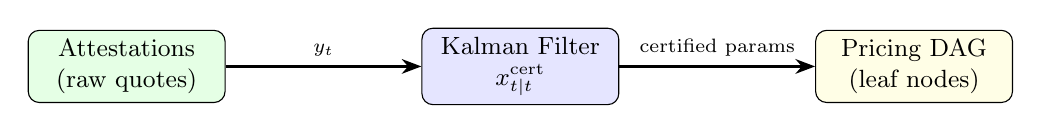
\begin{tikzpicture}[
    box/.style={draw, rounded corners, minimum width=2.5cm, minimum height=0.7cm, font=\small, align=center},
    arr/.style={-{Stealth[length=2.5mm]}, thick},
  ]
  \node[box, fill=green!10] (oracle) at (0,0) {Attestations\\(raw quotes)};
  \node[box, fill=blue!10] (kalman) at (5,0) {Kalman Filter\\$x_{t|t}^{\text{cert}}$};
  \node[box, fill=yellow!10] (dag) at (10,0) {Pricing DAG\\(leaf nodes)};

  \draw[arr] (oracle) -- node[above, font=\scriptsize] {$y_t$} (kalman);
  \draw[arr] (kalman) -- node[above, font=\scriptsize] {certified params} (dag);
\end{tikzpicture}
\end{center}

\noindent The Kalman filter runs as a dedicated Temporal workflow per calibrated object, signalling downstream pricing workflows when a new certified calibration is available---exactly like a market data node in the Pricing DAG.  The calibration workflow's cadence matches the observation frequency: real-time for liquid markets, periodic for illiquid curves.

\subsection{Broken States and Cross-Asset Coherence}

When multiple calibrated objects share information (e.g., SPX vol and SX5E vol are correlated), asynchronous updates can create broken states~\cite[\S7]{calibration_manifesto}: the stored pair $(\sigma_{\text{SPX}}, \sigma_{\text{SX5E}})$ no longer equals the conditional expectation given the full information set.  This is operationally important for cross-asset products (spread options, baskets).

The valuation stack handles this by: (1)~running joint Kalman filters for correlated parameters where cross-asset products exist, (2)~flagging pricing of cross-asset products as INDICATIVE when constituent calibrations are asynchronous beyond a configured threshold, and (3)~monitoring the innovation statistics for cross-asset consistency.

\clearpage
%==============================================================================
\section{The Pricing DAG}
\label{sec:pricing-dag}
%==============================================================================

Pricing is not a flat operation over independent instruments.  Dependencies form a directed acyclic graph---the \emph{Pricing DAG}.

\begin{definition}[Pricing DAG]
\label{def:pricing-dag}
The Pricing DAG is a directed acyclic graph $G = (N, E)$ where:
\begin{itemize}[nosep]
\item $N = N_U \cup N_M \cup N_C$: nodes are unit nodes ($N_U$), market data nodes ($N_M$), or calibration nodes ($N_C$, the Kalman filter outputs from Section~\ref{sec:calibration}).
\item $E \subseteq N \times N$: edge $(a, b)$ means ``$b$ requires a fresh value from $a$.''
\end{itemize}
\end{definition}

\noindent Calibration nodes sit between raw market data nodes and unit nodes: raw quotes $\to$ Kalman filter $\to$ calibrated parameters $\to$ pricing models $\to$ unit valuations.

\subsection{Construction Algorithm}

\begin{lstlisting}
BuildPricingDAG(unit_store: UnitStore) -> DAG:
    dag = empty DAG

    -- Step 1: Add market data nodes (leaf nodes)
    for each observable o referenced by any unit in unit_store:
        dag.add_node(o, type=MARKET_DATA, dependencies=[])

    -- Step 2: Add calibration nodes
    for each calibrated object c (yield curve, vol surface, ...):
        dag.add_node(c, type=CALIBRATION,
                     dependencies=c.input_observables())

    -- Step 3: Add unit nodes with dependencies
    for each unit u in unit_store where u.lifecycle_stage == ACTIVE:
        deps = u.smart_contract.pricing_dependencies()
        dag.add_node(u, type=UNIT, dependencies=deps)

    -- Step 4: Verify acyclicity
    if dag.has_cycle():
        raise DAGCycleError(dag.find_cycle())

    -- Step 5: Compute topological order
    dag.topo_order = topological_sort(dag)
    return dag
\end{lstlisting}

\begin{invariant}[Acyclicity]
The Pricing DAG is acyclic.  Enforced at unit registration: the Unit Store rejects units whose dependencies would create a cycle.
\end{invariant}

\subsection{DAG Topology by Instrument Class}

\begin{center}
\small
\begin{tabular}{l l l}
\toprule
\textbf{Instrument} & \textbf{Upstream dependencies} & \textbf{DAG depth} \\
\midrule
Cash (USD) & None & 0 \\
Equity spot & Exchange price feed & 1 \\
Yield curve (calibrated) & Deposit, futures, swap rates & 1 (calibration) \\
Vol surface (calibrated) & Option prices, ATM vol quotes & 1 (calibration) \\
Vanilla option & Spot, calibrated vol surface, calibrated rate curve & 2--3 \\
IRS & Calibrated USD yield curve & 2 \\
Structured note & Embedded option valuation, credit curve & 3+ \\
\bottomrule
\end{tabular}
\end{center}

\subsection{DAG Mutation}

The Pricing DAG changes when units are added or removed.  New units extend the DAG (with acyclicity verification); terminated units are removed.  Mid-cycle mutations take effect on the next cycle---a single cycle always operates on a frozen topology.

\clearpage
%==============================================================================
\section{Temporal Workflow Architecture for Pricing}
\label{sec:temporal}
%==============================================================================

\subsection{Design Principle: One Workflow per Unit}

Each unit in the Pricing DAG has a dedicated \texttt{PricingWorkflow(unit\_id)} that:
\begin{enumerate}[nosep]
\item waits for all upstream dependencies to signal fresh prices,
\item retrieves market data and unit state (lifecycle-before-valuation ordering),
\item invokes the pricer activity (base price),
\item dispatches Greek computation activities (bump-and-revalue fan-out),
\item runs PnL explain verification,
\item advances the FSM state (Section~\ref{sec:fsm}),
\item publishes the ValuationRecord,
\item updates the approximation service with fresh Greeks.
\end{enumerate}

\subsection{Cadence and Heterogeneous Compute}

\begin{center}
\small
\begin{tabular}{l r r l}
\toprule
\textbf{Instrument class} & \textbf{Cadence} & \textbf{Compute budget} & \textbf{Pricer type} \\
\midrule
Equity spot & 1--5s & $< 1$ms & Trivial (pass-through) \\
Vanilla option & 10--30s & 1--10ms & Analytical (Black-Scholes) \\
Exotic option & 1--5min & 1--30s & Monte Carlo / PDE \\
IRS & 30s--2min & 10--100ms & Curve bootstrapping \\
Bond & 30s--2min & 1--10ms & Yield-to-maturity \\
Structured note & 5--15min & 1--60s & Composite \\
\bottomrule
\end{tabular}
\end{center}

\subsection{DAG Signalling}

Reactive pricing via Temporal signals:
\begin{enumerate}[nosep]
\item Leaf node (market data feed or Kalman filter output) signals downstream unit workflows.
\item Unit workflow produces ValuationRecord, signals downstream dependents.
\item Downstream workflow checks freshness map: fire pricing only when ALL upstream nodes are fresh.
\end{enumerate}

\subsection{Workflow Pseudocode with FSM}

\begin{lstlisting}
PricingWorkflow(unit_id, cadence, dependencies):
    fsm_state = UNPRICED
    prev_record = None
    freshness = {dep: None for dep in dependencies}

    while unit_state(unit_id).lifecycle_stage == ACTIVE:
        -- Wait for upstream signals, lifecycle signals, or cadence timer
        await_signals_or_timer(freshness, cadence)

        -- Drain lifecycle signals (lifecycle-before-valuation)
        drain_lifecycle_signals(unit_id)

        if not all_fresh(freshness, cadence):
            continue

        -- T1 or T9 or T10: transition to PRICING
        fsm_state = PRICING

        -- Invoke base pricer
        result = await InvokePricer(unit_id, mkt_snap)
        if result.is_error():
            fsm_state = FAILED    -- T3
            await backoff_and_retry()
            continue

        fsm_state = PRICED        -- T2

        -- Compute Greeks
        greeks = await ComputeGreeks(unit_id, mkt_snap, result)
        raw_record = ValuationRecord(result, greeks, ...)

        -- T4: transition to EXPLAINING
        fsm_state = EXPLAINING
        explain = PnLExplain(prev_record, raw_record, market_moves)

        if explain.status == PASS:
            fsm_state = EXPLAINED  -- T5
            await PublishValuationRecord(raw_record.with_quality(FIRM))
            prev_record = raw_record
            await UpdateApproxCache(unit_id, raw_record)
            signal_downstream(unit_id, raw_record)
        else:
            fsm_state = QUARANTINED  -- T6
            await Quarantine(raw_record, explain)
            -- T7: retry with refreshed data
            retry_result = await RetryPricing(unit_id)
            if retry_result.explain_passes:
                fsm_state = EXPLAINED  -- T5 via T7
                await PublishValuationRecord(retry_result.record)
            else:
                fsm_state = STALE  -- T11
                await AlertRiskTeam(unit_id, explain)

        -- Staleness monitoring (T8)
        start_staleness_timer(cadence * staleness_factor)
\end{lstlisting}

\subsection{Timeout Configuration}

\begin{lstlisting}
PricerActivityOptions(instrument_class):
    match instrument_class:
        case EQUITY_SPOT:
            StartToCloseTimeout: 5s
            ScheduleToCloseTimeout: 30s
        case VANILLA_OPTION:
            StartToCloseTimeout: 30s
            ScheduleToCloseTimeout: 2min
        case EXOTIC_OPTION:
            StartToCloseTimeout: 5min
            ScheduleToCloseTimeout: 15min
        case IRS | BOND:
            StartToCloseTimeout: 2min
            ScheduleToCloseTimeout: 5min
    RetryPolicy:
        InitialInterval:    1s
        BackoffCoefficient: 2.0
        MaximumAttempts:    3
        NonRetryableErrors: [ModelNotFound, UnitNotActive]
\end{lstlisting}

\subsection{Task Queue Architecture}

\begin{center}
\small
\begin{tabular}{l l l}
\toprule
\textbf{Task queue} & \textbf{Instruments} & \textbf{Worker profile} \\
\midrule
\texttt{pricing-fast} & Equity spot, FX, cash & Low-latency, high-throughput \\
\texttt{pricing-analytical} & Vanilla options, bonds, IRS & Medium compute \\
\texttt{pricing-mc} & Exotic options, structured notes & GPU-enabled, high memory \\
\texttt{pricing-greeks} & Bump-and-revalue activities & Parallel, medium compute \\
\texttt{pricing-calibration} & Kalman filter updates & Medium compute, low latency \\
\texttt{pricing-workflow} & All PricingWorkflow orchestrators & Lightweight, many instances \\
\bottomrule
\end{tabular}
\end{center}

\subsection{Stale-Price Policy}

\begin{enumerate}
\item \textbf{Within cadence window}: workflow waits.  FSM stays in \textsc{Explained}.
\item \textbf{Beyond cadence ($\leq 3\times$)}: last FIRM price retained, \texttt{quality = STALE}.  FSM transitions to \textsc{Stale} via T8.
\item \textbf{Beyond $3\times$ cadence}: alert raised via obligation-liveness framework~\cite[\S14.7]{ledger}.
\end{enumerate}

\clearpage
%==============================================================================
\section{PnL Explain as Verification Gate}
\label{sec:pnl-explain}
%==============================================================================

Every new ValuationRecord must pass through PnL explain before publication.  This section connects the mathematical foundation of~\cite{pnl_explain,pnl_total_gamma} to the FSM transitions T4--T6.

\subsection{Mathematical Foundation}

For a pricing function $P$ treated as a cubic polynomial in market data vector $x \in \mathbb{R}^n$~\cite{pnl_explain,pnl_total_gamma}:

\paragraph{Ex post (exact for cubic $P$).}
\begin{equation}
\label{eq:pnl-expost}
P(x_2) - P(x_1) = \left\langle \frac{\Delta_{x_2} + \Delta_{x_1}}{2} \,\middle|\, x_2 - x_1 \right\rangle - \frac{1}{12}\langle x_2 - x_1 \,|\, (\Gamma_{x_2} - \Gamma_{x_1}) \,|\, x_2 - x_1 \rangle
\end{equation}

\paragraph{Decomposition into three orders.}
\begin{equation}
\label{eq:pnl-decomp}
P(x_2) - P(x_1) = \underbrace{\langle \Delta_{x_1} \,|\, h \rangle}_{\text{1st order}} + \underbrace{\left\langle \frac{\Delta_{x_2} - \Delta_{x_1}}{2} \,\middle|\, h \right\rangle}_{\text{2nd order}} - \underbrace{\frac{1}{12}\langle h \,|\, (\Gamma_{x_2} - \Gamma_{x_1}) \,|\, h \rangle}_{\text{3rd order}}
\end{equation}

\noindent The Greeks $\Delta_{x_1}$ and $\Delta_{x_2}$ must come from the same model $\mathcal{M}$.  When using instruments with smile-dependent volatility, these must be the \emph{total} Greeks (Section~\ref{sec:total-greeks}).

\begin{remark}[Model Consistency in PnL Explain]
\label{rem:model-consistency}
Using model $\mathcal{M}_1$'s Greeks to explain model $\mathcal{M}_2$'s price change produces a residual that is a model artefact.  When a model transition occurs, the PnL explain gate is suspended for the transition record, and the model change generates an explicit ``model change PnL'' reported separately.
\end{remark}

\subsection{The PnL Explain Function}

\begin{definition}[PnL Explain]
\label{def:pnl-explain}
\begin{lstlisting}
pnl_explain(
    prev:         ValuationRecord,    -- FSM was EXPLAINED
    curr:         ValuationRecord,    -- FSM is PRICED
    market_moves: MarketDataDelta,
    cashflows:    List[Move]          -- lifecycle cash flows
) -> ExplainResult

precondition: prev.model_id == curr.model_id
\end{lstlisting}

The computation:
\begin{lstlisting}
    total_pnl = curr.dirty_price - prev.dirty_price
    explained = (
        prev.greeks.delta * market_moves.spot_change
      + 0.5 * prev.greeks.gamma * market_moves.spot_change^2
      + prev.greeks.vega * market_moves.vol_change
      + prev.greeks.theta * dt
      + prev.greeks.rho * market_moves.rate_change
      + sum(cf.amount for cf in cashflows))
    unexplained = total_pnl - explained
    if abs(unexplained) < tolerance(unit_id):
        return ExplainResult(status=PASS, ...)   -- enables T5
    else:
        return ExplainResult(status=FAIL, ...)   -- triggers T6
\end{lstlisting}
\end{definition}

\subsection{Tolerances}

\begin{center}
\small
\begin{tabular}{l l}
\toprule
\textbf{Instrument class} & \textbf{Tolerance (per unit notional)} \\
\midrule
Equity spot & \$0.01 (essentially zero) \\
Vanilla option & 1\% of option premium \\
Exotic option & 2\% of option premium \\
IRS & 0.5 basis points of notional \\
Bond & 0.1\% of face value \\
\bottomrule
\end{tabular}
\end{center}

\subsection{Failure Handling (FSM transitions T6, T7, T11)}

When PnL explain fails (T6: \textsc{Explaining} $\to$ \textsc{Quarantined}):
\begin{enumerate}
\item \textbf{Quarantine.}  Candidate record held; previous FIRM price remains current.
\item \textbf{Alert.}  Event-triggered obligation with deadline $3\times$ cadence.
\item \textbf{Retry (T7).}  Re-invoke with refreshed market data or alternative model.
\item \textbf{Manual override.}  If automated retries fail, manual price with \texttt{quality = INDICATIVE}.
\item \textbf{Exhaustion (T11).}  Last-known-good with \texttt{quality = STALE}.
\end{enumerate}

\clearpage
%==============================================================================
\section{Continuous Approximate Pricing}
\label{sec:approx-pricing}
%==============================================================================

\begin{principle}[Price Availability]
\label{princ:price-availability}
At any time $t$, for any active unit $u$ in FSM state \textsc{Explained}, a price is always available via Taylor expansion from the last FIRM valuation.
\end{principle}

\subsection{The Taylor Approximation Formula}

Let $t_{\mathrm{last}}$ be the timestamp of the last FIRM valuation (FSM entered \textsc{Explained}).  At time $t > t_{\mathrm{last}}$:
\begin{equation}
\label{eq:taylor-approx}
\boxed{
P_{\mathrm{approx}}(u, t) = P_{\mathrm{FIRM}}(u) + \delta \cdot \Delta S(t) + \tfrac{1}{2}\,\Gamma \cdot \Delta S(t)^2 + \nu \cdot \Delta\sigma(t) + \Theta \cdot \Delta t + \rho \cdot \Delta r(t)
}
\end{equation}

For instruments with multiple risk factors:
\begin{equation}
P_{\mathrm{approx}}(u, t) = P_{\mathrm{FIRM}}(u) + \langle \Delta_{t_{\mathrm{last}}} \,|\, \Delta x(t) \rangle + \tfrac{1}{2}\langle \Delta x(t) \,|\, \Gamma_{t_{\mathrm{last}}} \,|\, \Delta x(t) \rangle
\end{equation}

\subsection{Properties}

\begin{enumerate}
\item \textbf{$O(1)$ per unit.}  Multiply cached Greeks by market moves.
\item \textbf{Accuracy degrades} with time and large moves.  Self-correcting on next full reprice.
\item \textbf{Quality = APPROXIMATE.}  Distinguished from FIRM and STALE.
\item \textbf{FSM context.}  Available only in state \textsc{Explained}.  When the unit transitions to \textsc{Stale}, the approximation is no longer trusted.
\end{enumerate}

\subsection{Official PnL Uses FIRM Prices Only}

\begin{principle}[FIRM-Only PnL]
\label{princ:firm-pnl}
The official PnL computation uses only FIRM ValuationRecords at configured valuation points.  APPROXIMATE prices are acceptable for intraday risk monitoring but not for official PnL, regulatory reports, or end-of-day flash.
\end{principle}

\clearpage
%==============================================================================
\section{The Valuation Store}
\label{sec:valuation-store}
%==============================================================================

ValuationRecords are stored in a valuation store indexed by \texttt{(unit\_id, timestamp, model\_id)}.  The store is append-only within a pricing cycle.

Five consumers: (1)~Ledger PnL computation (reads \texttt{dirty\_price}, FIRM only), (2)~obligation-liveness executor (CSA margin), (3)~risk pipeline (Greeks for limits), (4)~PnL explain (reads previous FIRM record), (5)~approximation service (reads latest FIRM record with Greeks).

Point-in-time queries support time travel: \texttt{snapshot\_at($t$)} returns the latest record per unit with timestamp $\leq t$.

\clearpage
%==============================================================================
\section{Edge Cases}
\label{sec:edge-cases}
%==============================================================================

\subsection{Market Data Gap}
Market data unavailability: downstream workflows wait or proceed with stale data.  FSM: units depending on stale market data transition T8 to \textsc{Stale}.

\subsection{Model Failure}
Pricer crash, timeout, or NaN: FSM transition T3 to \textsc{Failed}, then T10 retry with backoff.  Fallback model hierarchy per instrument class.

\subsection{DAG Mutation Mid-Cycle}
New trades extend the DAG on the next cycle; terminated units are removed.

\subsection{Monte Carlo Determinism}
MC pricers use deterministic seeds: \texttt{seed = hash(market\_data\_snap, unit\_id)}.  Same inputs produce same outputs, satisfying purity~\cite[\S7.7]{ledger}.

\subsection{Taylor Approximation During Large Moves}
Large market moves ($>5\%$ since last FIRM): trigger immediate full reprice for affected units; APPROXIMATE prices flagged with ``large move'' warning; risk pipeline applies prudential haircut.

\clearpage
%==============================================================================
\section{Worked Example: Complete Valuation Cycle}
\label{sec:worked-example}
%==============================================================================

\subsection{Setup}

Three-instrument portfolio: NVDA spot (cadence 5s), NVDA Jun~2026 900~Call (cadence 30s), structured note embedding the call (cadence 5min).

\noindent\textbf{Previous valuations (14:29:30 UTC):}
\begin{center}
\small
\begin{tabular}{l r r r r r l}
\toprule
\textbf{Unit} & \textbf{Price} & \textbf{$\delta$} & \textbf{$\gamma$} & \textbf{$\nu$} & \textbf{$\theta$} & \textbf{FSM state} \\
\midrule
NVDA & \$908.00 & 1.000 & --- & --- & --- & \textsc{Explained} \\
NVDA-C-Jun26-900 & \$68.20 & 0.571 & 0.0039 & 0.298 & $-0.138$ & \textsc{Explained} \\
SN-NVDA-001 & \$102.30 & --- & --- & --- & --- & \textsc{Explained} \\
\bottomrule
\end{tabular}
\end{center}

\subsection{14:29:45 UTC --- Approximate Pricing (FSM: \textsc{Explained})}

NVDA spot: \$910.20 ($\Delta S = +\$2.20$).  Vol: 42.1\% ($\Delta\sigma = +0.3\%$).
\begin{align*}
P_{\mathrm{approx}}(\text{NVDA-C}) &= 68.20 + 0.571 \times 2.20 + \tfrac{1}{2} \times 0.0039 \times 2.20^2 + 0.298 \times 0.3 - 0.138 \times \tfrac{15}{365} \\
&= \$69.55 \quad\text{(quality = APPROXIMATE, FSM: \textsc{Explained})}
\end{align*}

\subsection{14:30:00 UTC --- Full Reprice Cycle}

Fresh data: NVDA \$912.50, vol 42.3\%, rate 5.20\%.  All units transition through the FSM:

\paragraph{NVDA spot.}  FSM: \textsc{Explained} $\xrightarrow{\text{T1/T9}}$ \textsc{Pricing} $\xrightarrow{\text{T2}}$ \textsc{Priced} $\xrightarrow{\text{T4}}$ \textsc{Explaining}.  PnL explain: $|912.50 - 908.00 - 1.0 \times 4.50| = 0$.  \textsc{Pass}.  $\xrightarrow{\text{T5}}$ \textsc{Explained}.

\paragraph{NVDA Call.}  BSM output: \$72.85, $\delta = 0.583$, $\gamma = 0.0041$.  FSM: \textsc{Explained} $\to$ \textsc{Pricing} $\to$ \textsc{Priced} $\to$ \textsc{Explaining}.  Explained PnL = \$4.159; actual = \$4.65; unexplained = \$0.49 $<$ \$1.00 tolerance.  \textsc{Pass}.  $\to$ \textsc{Explained}.

\paragraph{Structured note.}  $P = 100 \times 72.85 / 71.00 = \$102.61$.  Unexplained $\approx \$0.00$.  \textsc{Pass}.  $\to$ \textsc{Explained}.

\subsection{Portfolio Valuation}

\begin{align*}
V_{14:30:00} &= 100 \times 912.50 + 50 \times 72.85 + 200 \times 102.61 = \$115{,}414.50 \\
\mathrm{PnL} &= 115{,}414.50 - 114{,}670.00 = +\$744.50
\end{align*}
Path-independent per~\cite[\S4.3]{ledger}.

\clearpage
%==============================================================================
\section{Consistency with the Lifecycle Engine}
\label{sec:lifecycle-consistency}
%==============================================================================

\subsection{The Price Function Depends on Unit State}

\begin{principle}[State-Dependent Pricing]
\label{princ:state-dep-pricing}
The price function is:
\begin{equation}\label{eq:price-func}
\boxed{P_t(u) = P\bigl(u,\; \mathrm{state}_t(u),\; \mathrm{market\_data}_t\bigr)}
\end{equation}
where $\mathrm{state}_t(u)$ is the unit state dictionary from the lifecycle engine at time~$t$.  A pricer invocation without the current unit state is ill-defined.
\end{principle}

\noindent This is the formal definition of the price function.  The scalar compatibility principle (Principle~\ref{princ:scalar-compat}) is preserved: \texttt{dirty\_price} is still the $P_t(u)$ consumed by the PnL computation.

\subsection{The Lifecycle-Valuation Ordering Protocol}

\begin{principle}[Lifecycle-Before-Valuation]
\label{princ:lifecycle-before-val}
For any unit $u$, all pending lifecycle events must be processed before the next valuation cycle begins.  The FSM transition T1/T9 (entering \textsc{Pricing}) requires:
\begin{enumerate}[nosep]
\item[(a)] fresh market data for all upstream dependencies, AND
\item[(b)] confirmation that no pending lifecycle events exist for $u$.
\end{enumerate}
\end{principle}

This is implemented via Temporal signals: the lifecycle workflow signals the pricing workflow after each event.  The pricing workflow drains all pending lifecycle signals before reading unit state.

\subsection{Lifecycle Events and the FSM}

Material lifecycle events (Definition~\ref{def:repricing-class}) force an FSM transition:
\begin{itemize}[nosep]
\item If in \textsc{Explained}: transition to \textsc{Pricing} (bypass T8, immediate reprice).
\item If in \textsc{Stale}: transition to \textsc{Pricing} (lifecycle event provides the trigger for T9).
\item Cached Greeks are invalidated; Taylor approximation returns \textsc{Stale} until reprice completes.
\end{itemize}

\begin{definition}[Repricing Classification]
\label{def:repricing-class}
A lifecycle event is \textbf{material} if it changes $P(u, \mathrm{state}_t(u), \mathrm{market\_data}_t)$ for fixed market data.  Material events: coupon payment, exercise, expiry, barrier breach, settlement, partial return.  Non-material events: margin calls, collateral substitution, reporting.
\end{definition}

\subsection{Taylor Approximation Invalidation}

Lifecycle events create price discontinuities not captured by Greeks:
\begin{center}
\small
\begin{tabular}{l l}
\toprule
\textbf{Event} & \textbf{Discontinuity} \\
\midrule
Coupon payment & Dirty price drops by coupon amount \\
Ex-dividend & Equity price drops by dividend amount \\
Option exercise/expiry & Price $\to$ intrinsic or 0 \\
Barrier knock-in/out & Price jumps \\
\bottomrule
\end{tabular}
\end{center}

On material lifecycle event: invalidate Greeks cache, return \texttt{quality = STALE} until reprice, optionally apply closed-form adjustment ($P_{\text{adj}} = P_{\text{last}} - \text{coupon}$) with \texttt{quality = APPROXIMATE}.

\subsection{Extended Pricing DAG}

The extended DAG $G' = (N, E_M \cup E_S)$ distinguishes market data edges ($E_M$) from state dependency edges ($E_S$).  State edges are self-loops (unit state to unit pricer) and do not affect topological order.

\subsection{Worked Example: Bond Coupon Payment}

\paragraph{Setup.}  Corporate bond, 5\% annual coupon, semi-annual \$2.50.  Pre-coupon FIRM: dirty \$102.50, clean \$100.00, accrued \$2.50.

\paragraph{Sequence.}
\begin{enumerate}[nosep]
\item Lifecycle event fires (16:05): coupon paid, accrued resets.  Signal sent to pricing workflow.
\item Taylor invalidated: approximate price = \$102.50 $-$ \$2.50 = \$100.00 (APPROXIMATE).
\item Pricing workflow fires (16:06): post-coupon state, yield +2~bp.  New dirty price \$99.93.
\item PnL explain: total $-$\$2.57 = coupon ($-$\$2.50) + theta (+\$0.014) + duration ($-$\$0.084).  Unexplained \$0.00.  \textsc{Pass}.  FSM $\to$ \textsc{Explained}.
\end{enumerate}

\clearpage
%==============================================================================
\section{Production Scalability Analysis}
\label{sec:scalability}
%==============================================================================

\subsection{Workflow Execution Volume}

The one-workflow-per-unit design creates $|\mathcal{U}|$ concurrent Temporal workflows.  The workflow execution rate depends on the instrument mix and cadence:

\begin{center}
\small
\begin{tabular}{l r r r r}
\toprule
\textbf{Instrument class} & \textbf{Count} & \textbf{Cadence} & \textbf{Cycles/min} & \textbf{Executions/min} \\
\midrule
Equity spot & 10{,}000 & 5s & 12 & 120{,}000 \\
Vanilla options & 50{,}000 & 30s & 2 & 100{,}000 \\
Exotic options & 5{,}000 & 5min & 0.2 & 1{,}000 \\
IRS / bonds & 20{,}000 & 1min & 1 & 20{,}000 \\
Structured notes & 5{,}000 & 10min & 0.1 & 500 \\
Calibration workflows & 100 & 10s & 6 & 600 \\
\midrule
\textbf{Total} & \textbf{90{,}100} & & & $\approx$\textbf{242{,}100} \\
\bottomrule
\end{tabular}
\end{center}

At 100{,}000 units with a weighted-average cadence of approximately 25 seconds, the system generates approximately 240{,}000 workflow task completions per minute, or approximately 4{,}000 per second.

\subsection{Temporal Cluster Sizing}

Each pricing cycle involves 3--5 Temporal activities (market data retrieval, base pricing, Greek computation fan-out, PnL explain, publication).  At 240K cycles/min with 4 activities each, the cluster processes approximately 16{,}000 activities per second.

\paragraph{Workflow workers (\texttt{pricing-workflow}).}  Each workflow is lightweight (state machine logic, signal handling).  A single worker can handle 1{,}000--5{,}000 concurrent workflows.  At 90{,}000 active workflows: 20--90 workflow workers.

\paragraph{Activity workers.}  Activity compute varies by queue:
\begin{itemize}[nosep]
\item \texttt{pricing-fast}: 120K activities/min, $<1$ms each.  2--4 workers.
\item \texttt{pricing-analytical}: 100K activities/min, 1--10ms each.  10--20 workers.
\item \texttt{pricing-mc}: 1{,}000 activities/min, 10--30s each.  50--100 GPU workers.
\item \texttt{pricing-greeks}: proportional to analytical + MC.  20--50 workers.
\item \texttt{pricing-calibration}: 600 activities/min.  2--4 workers.
\end{itemize}

\paragraph{Temporal server.}  The Temporal server cluster (frontend, history, matching services) must handle 16K activities/second dispatch rate.  A horizontally scaled Temporal deployment with 3--5 history shards and Cassandra/MySQL backend handles this comfortably---Temporal's published benchmarks show 10K--50K activities/second per shard.

\subsection{History Management}

Long-running pricing workflows (lifetime = unit lifetime, potentially years) accumulate event history.  The \texttt{ContinueAsNew} pattern~\cite[\S14.12]{ledger} resets history every $N$ cycles (configurable, e.g., 1{,}000 cycles or 24 hours), carrying forward only the FSM state, previous FIRM record, and freshness map.  This bounds per-workflow history to a manageable size.

\subsection{Scalability Summary}

\begin{center}
\small
\begin{tabular}{l r}
\toprule
\textbf{Metric} & \textbf{Value at 100K units} \\
\midrule
Concurrent workflows & $\sim$90{,}000 \\
Workflow executions / minute & $\sim$240{,}000 \\
Activity dispatches / second & $\sim$16{,}000 \\
Workflow workers & 20--90 \\
Activity workers (total) & 85--180 \\
Temporal server shards & 3--5 \\
Peak memory (workflow state) & $\sim$9 GB (100 KB/workflow) \\
\bottomrule
\end{tabular}
\end{center}

The architecture scales horizontally: doubling the unit count doubles the worker pool but does not change the per-unit resource consumption.  The bottleneck is MC pricer compute for exotic options, addressed by GPU worker pools and cadence management (longer cadence for less liquid exotics).

\clearpage
%==============================================================================
\section{Interaction Summary}
\label{sec:interactions}
%==============================================================================

\begin{center}
\small
\begin{tabular}{l p{3.5cm} p{6.5cm}}
\toprule
\textbf{Component} & \textbf{Interface} & \textbf{Data flow} \\
\midrule
Move stream~\cite[\S8]{ledger} & Read-only & Valuation store reads wallet balances for $V_t$. \\
Unit Store~\cite[\S3]{ledger} & Read-only & DAG constructed from \texttt{pricing\_dependencies()}. \\
Calibration engine & Bidirectional & Kalman filter reads raw quotes, produces certified params for DAG leaf nodes. \\
Obligation-liveness~\cite[\S14.7]{ledger} & Write (alerts) & PnL explain failures and staleness create obligations. \\
Temporal~\cite[\S14]{ledger} & Bidirectional & PricingWorkflows, calibration workflows, Greek activities. \\
Lifecycle engine~\cite[\S7]{ledger} & Read + signals & Unit state for pricing; lifecycle signals for ordering and invalidation. \\
\bottomrule
\end{tabular}
\end{center}

\clearpage
%==============================================================================
\section{Conclusion and Open Problems}
\label{sec:conclusion}
%==============================================================================

This document specifies the valuation layer that produces the price function $P_t$ consumed by the Ledger framework.  Version~1.0 makes five contributions beyond v0.2:

\begin{enumerate}
\item \textbf{Valuation lifecycle FSM} (Section~\ref{sec:fsm}): eight states, twelve transitions, every state defined, every transition guarded.  The FSM makes explicit the progression from market data arrival through pricing, verification, and publication.

\item \textbf{Kalman filter for market data calibration} (Section~\ref{sec:calibration}): the full predict-update cycle with innovation-based gating, no-arbitrage constraints, and integration with the Pricing DAG as calibration nodes.

\item \textbf{Greeks, parameters, and the sensitivity Jacobian} (Section~\ref{sec:greeks}): a pricing model has parameters assumed to be martingales; Greeks are partial derivatives holding parameters constant.  The scalar ``vega'' is shown to vanish for multi-parameter models, replaced by the sensitivity Jacobian---a vector in $\mathbb{R}^n$ where $n$ is the parameter count.  PnL attribution with the full Jacobian explicitly decomposes the ``parameter PnL'' that was previously lumped into the unexplained residual.  Black--Scholes vs.\ local vol delta worked concretely, total gamma with vanna/volga/vega-curvature, the toxic product boundary, the consensus protocol for multi-model disagreement, and practical computation (analytical, bump-and-revalue, AAD, pathwise/likelihood ratio).

\item \textbf{Formal price function} (Section~\ref{sec:lifecycle-consistency}): $P(u, \mathrm{state}_t(u), \mathrm{market\_data}_t)$ as a formal definition, lifecycle events as FSM transitions, Taylor approximation positioned in the FSM.

\item \textbf{Production scalability analysis} (Section~\ref{sec:scalability}): 100K units at mixed cadence yields $\sim$240K workflow executions/minute, within Temporal cluster capacity with 90--180 workers and 3--5 server shards.
\end{enumerate}

\subsection{Open Problems}

\paragraph{Intraday curve bootstrapping.}  Should bootstrapping be a Temporal workflow in the Pricing DAG?  The Kalman filter (Section~\ref{sec:calibration}) provides a natural answer: yes, as a calibration node.  The open question is whether the bootstrapping algorithm itself (cubic spline, piecewise linear) should be inside the Kalman state or outside it.

\paragraph{Cross-asset correlation.}  PnL explain operates per-unit.  Portfolio-level attribution requires cross-asset Greeks.  The joint Kalman filter (Section~\ref{sec:calibration}) addresses the calibration side; extending to portfolio-level PnL explain is future work.

\paragraph{Model risk framework.}  The multi-model consensus (Section~\ref{sec:consensus}) specifies the operational protocol.  Formal model risk reserve calculations, dual-valuation regulatory requirements, and automated model comparison are future work.

\paragraph{Adaptive cadence.}  The fixed cadence per instrument class (Section~\ref{sec:temporal}) is a simplification.  Instruments approaching barriers, near expiry, or with rapidly changing Greeks need shorter cadences.  Formal error bounds on the Taylor approximation and adaptive cadence selection are open.

\paragraph{Scaling beyond 1M units.}  The scalability analysis (Section~\ref{sec:scalability}) covers 100K units.  Scaling to millions of listed derivatives requires workflow batching (multiple units per workflow), hierarchical DAG evaluation, and potentially moving from one-workflow-per-unit to one-workflow-per-portfolio-slice.

\clearpage
%==============================================================================
\begin{thebibliography}{99}

\bibitem{ledger}
R.~Delloye, ``The Ledger: A Closed-System Framework for Financial Settlement---Unified Design Specification: Architecture, Lifecycle, and CDM Integration,'' v10.3, March~2026.

\bibitem{pnl_explain}
R.~Delloye, ``On the Consistency of Derivative P\&L Across Sequential Calculations Using Polynomial Approximations,'' 2026.

\bibitem{pnl_total_gamma}
R.~Delloye, ``P\&L Attribution and Total Greeks: A Unified Framework via Polynomial Approximation and Smile-Adjusted Sensitivities,'' 2026.

\bibitem{total_gamma}
R.~Delloye, ``Gamma Adjustment with Quadratic Volatility: Final Derivation,'' 2026.

\bibitem{calibration_manifesto}
R.~Delloye, ``Market Data Calibration Manifesto,'' March~2026.

\bibitem{implied_vol}
R.~Delloye, ``Modeling Implied Volatility via Kernel-Based Representations of the Curve,'' 2026.

\bibitem{implied_local_vol}
R.~Delloye, ``Implied and Local Volatility via Kernel-Based Curve Representations,'' 2026.

\bibitem{loc_vol}
R.~Delloye, ``Local Volatility in the Context of Quadratic Implied Volatility in Log-Moneyness,'' 2026.

\bibitem{control_variate}
R.~Delloye, ``Pricing Complex Derivatives via Regression-Based Monte Carlo and Surrogate Models,'' 2026.

\end{thebibliography}

\end{document}
